\MainChapter{Diseño de la solución}{\topBanner}\label{cap:disenio-solucion}
\vspace*{0.7cm}

\section{Modelado del sistema en ArchiMate}\label{sec:archimate-modelado}

ArchiMate es un lenguaje de modelado estandarizado por~\textit{The Open Group} que permite representar de manera estructurada los componentes y relaciones que conforman una arquitectura empresarial. Su utilización permite establecer una visión integrada de los elementos de negocio, aplicación y tecnología, facilitando la representación de las relaciones existentes entre las necesidades de la organización, los servicios de información y la infraestructura que los soporta~\citep{opengroup_archimate_overview}.

En el presente proyecto, ArchiMate se utilizó para modelar la arquitectura propuesta para el servicio de directorio del grupo de investigación \ac{GRID}. El modelado permitió representar la relación entre los actores que hacen uso de los servicios, los servicios tecnológicos que requieren mecanismos de autenticación y autorización, y los componentes que conforman la solución de directorio seleccionada. De esta manera, se estableció una representación de la solución que permite visualizar cómo el servicio de directorio se integra con los diferentes servicios considerados dentro del alcance del proyecto.

El modelo contempla principalmente los elementos relacionados con la gestión centralizada de identidades y el acceso a los servicios integrados, así como los componentes tecnológicos necesarios para proporcionar dicha funcionalidad. En este contexto, se representa a FreeIPA como componente central de la solución, encargado de proporcionar los servicios de directorio y gestión de identidades sobre los cuales se soporta la autenticación de los servicios integrados.

La representación mediante ArchiMate permitió, además, establecer las relaciones entre los diferentes elementos de la arquitectura y proporcionar una visión general de la solución, facilitando la comprensión de su estructura y de las interacciones entre sus componentes. En el Anexo~\ref{tab:elementos-negocio-archimate} se especifica el significado de los principales elementos y relaciones utilizados en el modelado.

\section{Metodología de diseño}\label{sec:metodologia-diseno}

El diseño de la solución se estructuró en dos componentes complementarios: el diseño mediante diagramas y el diseño de las configuraciones. Esta división permitió abordar la solución desde una perspectiva arquitectónica y, posteriormente, desde una perspectiva técnica, manteniendo una relación entre la representación de los componentes y las configuraciones necesarias para su implementación.

La primera parte correspondió al diseño mediante diagramas, en el cual se representaron los componentes que conforman la solución y las relaciones existentes entre ellos. Para ello, se empleó ArchiMate como lenguaje de modelado, de acuerdo con los elementos y relaciones definidos para representar la arquitectura propuesta.

La segunda parte correspondió al diseño de las configuraciones, en la cual se especificaron los aspectos técnicos necesarios para materializar la arquitectura definida en los diagramas. Esta parte contempló las configuraciones requeridas para el funcionamiento del servicio de directorio, así como aquellas necesarias para su integración con los servicios considerados dentro del alcance.

De esta manera, ambas partes del diseño se complementaron: los diagramas permitieron definir y comunicar la estructura de la solución, mientras que el diseño de configuraciones permitió establecer los aspectos técnicos necesarios para su posterior implementación.

\section{Diagramas}\label{sec:diagramas}

\subsection{Vista de negocio}

\subsubsection{Vista cooperación de actores}

La \autoref{fig:actor-cooperation} presenta la vista de cooperación de actores, cuyo propósito es representar las interacciones entre los diferentes actores organizacionales que participan en la operación del Grupo de Investigación \ac{GRID} y la forma en que colaboran para la prestación de los servicios académicos y administrativos. Esta vista permite identificar las responsabilidades de cada actor, los flujos de información y los principales artefactos documentales que soportan el funcionamiento de los procesos de negocio.

En el diagrama se observa la participación de los actores externos, representados por los estudiantes, docentes y administradores, así como los actores internos que conforman el grupo de investigación \ac{GRID}, entre ellos la directiva, el área de cursos de ingesis y el área de relaciones contractuales. Las relaciones establecidas evidencian las actividades de cooperación necesarias para el desarrollo de los cursos, la gestión administrativa y la vinculación del personal docente

\begin{figure}[H]
	\centering
	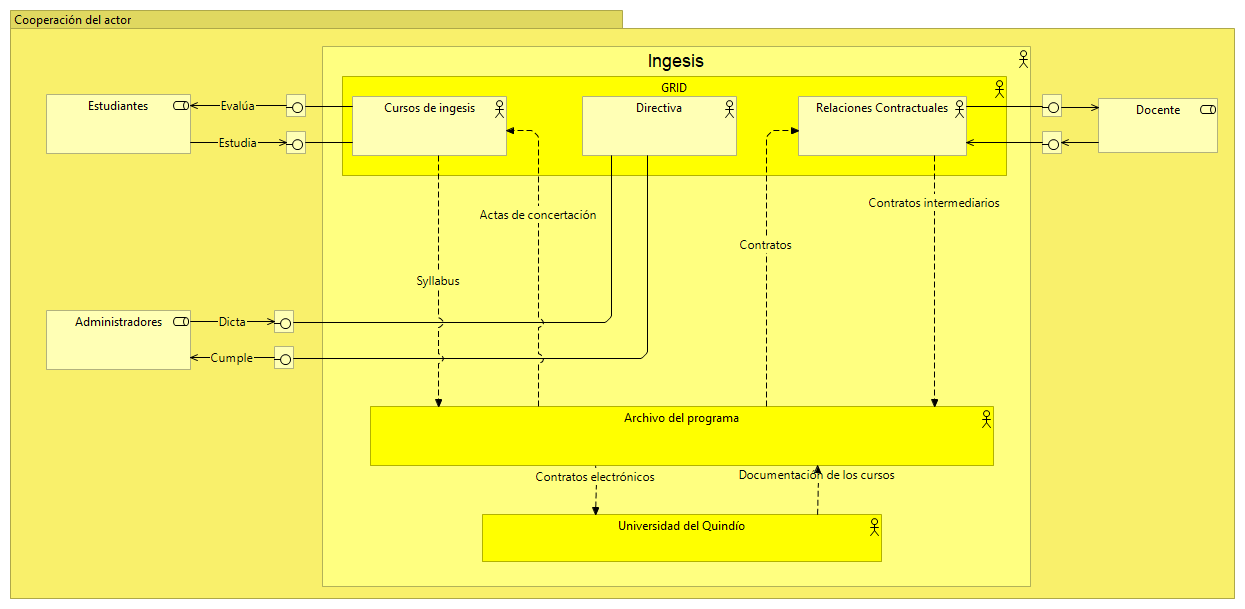
\includegraphics[width=0.9\textwidth]{imagenes/figuras/II-desarrollo-metodologico/disenio/actor-cooperation.png}
	\caption{vista de cooperación de actores}
	\label{fig:actor-cooperation}
\end{figure}

\subsubsection{Vista de proceso de negocio}

La \autoref{fig:business-process} presenta la vista de proceso de negocio, cuyo propósito es modelar las actividades que conforman el ciclo de gestión de identidades y el proceso de autenticación de usuarios dentro de la solución propuesta. Esta vista permite comprender la secuencia lógica de las operaciones, los responsables involucrados y la información que interviene en cada etapa del proceso, independientemente de los componentes tecnológicos que posteriormente las implementan.

En el diagrama se identifican dos procesos principales. El primero corresponde a la gestión de usuarios, el cual inicia con la solicitud de creación o actualización de una cuenta por parte del administrador de tecnologías de la información. A continuación, se realiza la validación de la información suministrada, el procesamiento de los datos y la asignación de grupos y permisos, actividades que permiten generar o actualizar el registro del usuario y su pertenencia a los grupos correspondientes, de acuerdo con las políticas institucionales definidas. Como resultado del proceso se obtiene un usuario correctamente aprovisionado y preparado para acceder a los servicios institucionales.

El segundo proceso corresponde a la gestión de accesos, el cual inicia cuando un usuario solicita el inicio de sesión en alguno de los servicios integrados. Durante este proceso se validan las credenciales presentadas y posteriormente se verifican los permisos asociados a la cuenta, consultando los registros de usuarios, grupos y las políticas de acceso definidas. Si las validaciones son satisfactorias, el usuario obtiene acceso al servicio solicitado; en caso contrario, la autenticación o autorización es rechazada.

\begin{figure}[H]
	\centering
	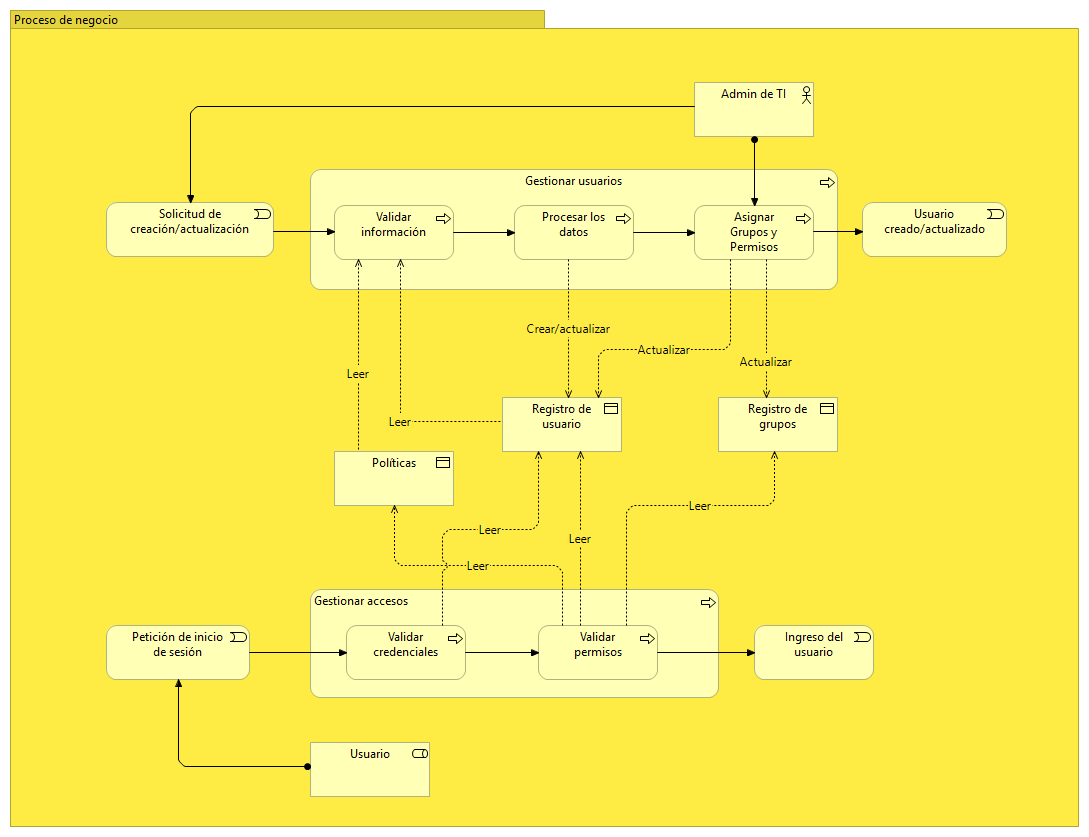
\includegraphics[width=0.9\textwidth]{imagenes/figuras/II-desarrollo-metodologico/disenio/business-process.png}
	\caption{vista de proceso de negocio}
	\label{fig:business-process}
\end{figure}

\subsection{Vista de aplicación}

La \autoref{fig:application-services} presenta la vista de componentes y servicios de aplicación, cuyo propósito es describir la estructura lógica de la solución implementada y las interacciones entre los componentes que conforman el servicio de directorio centralizado. Esta vista permite identificar cómo cada componente de FreeIPA coopera para proporcionar los servicios de autenticación, autorización y administración de identidades consumidos por las aplicaciones institucionales.

En el núcleo de la arquitectura se encuentra FreeIPA, representado como el contenedor lógico que integra los diferentes componentes responsables de la gestión de identidades. Entre estos se encuentra 389 Directory Server, encargado del almacenamiento y administración de la información del directorio \ac{LDAP}; Kerberos (\acs{KDC}), responsable de la autenticación mediante tickets y de la validación de identidades; Dogtag Certificate Authority, encargado de la emisión y administración de certificados digitales; Policy Engine, que implementa la evaluación de las políticas de autorización y control de acceso; y Web \acs{UI} + \ac{API}, que proporciona la interfaz administrativa y los servicios necesarios para la gestión del directorio.

El diagrama también muestra la cooperación entre estos componentes. El servidor de directorio constituye el repositorio central de identidades, siendo consultado por el servicio Kerberos durante los procesos de autenticación y por el motor de políticas para la evaluación de las reglas de autorización. De igual forma, la interfaz de administración consulta y actualiza la información almacenada en el directorio, mientras que la autoridad certificadora interactúa con esta para gestionar los certificados digitales asociados a usuarios y servicios.

\begin{figure}[H]
	\centering
	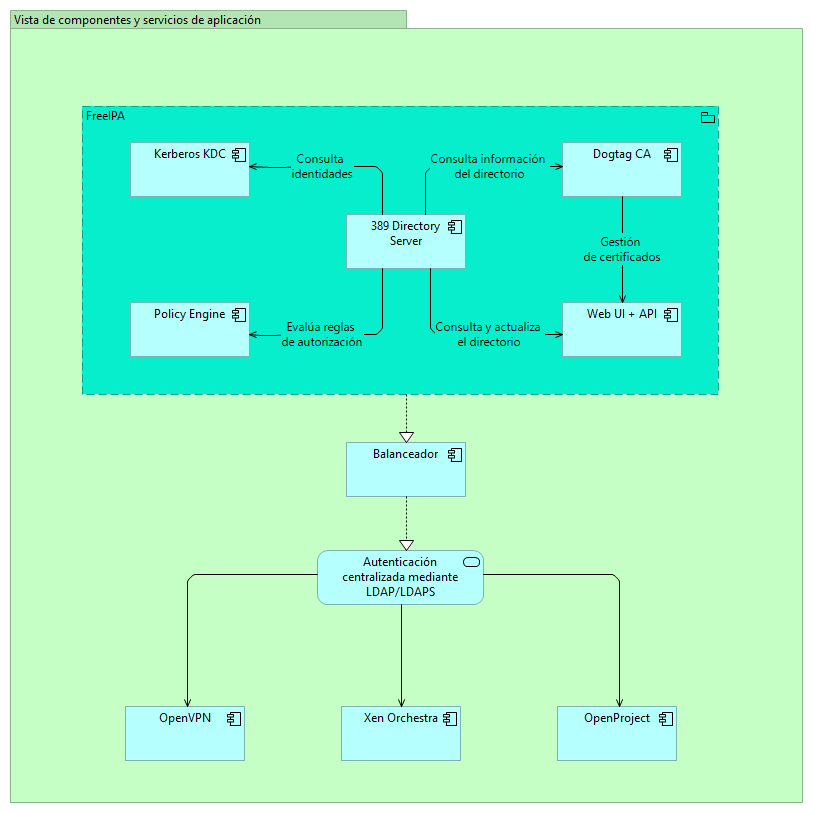
\includegraphics[width=0.9\textwidth]{imagenes/figuras/II-desarrollo-metodologico/disenio/application-services.png}
	\caption{vista de componentes y servicios de aplicación}
	\label{fig:application-services}
\end{figure}

\subsection{Capa de implementación}

La \autoref{fig:implementation} presenta la vista de implementación, cuyo propósito es representar el despliegue físico y lógico de la solución dentro de la infraestructura tecnológica del Grupo de Investigación \ac{GRID}. Esta vista muestra la distribución de los servicios sobre el hipervisor, la organización de las máquinas virtuales, los mecanismos de comunicación entre ellas y los componentes que soportan la autenticación centralizada.

La arquitectura se encuentra desplegada sobre un hipervisor XCP-ng, el cual aloja las máquinas virtuales que conforman la solución. Estas se agrupan en dos dominios funcionales: el primero corresponde a los servidores de autenticación, donde se encuentran el servidor principal, el servidor réplica de FreeIPA y el balanceador de carga; el segundo agrupa las aplicaciones consumidoras, conformadas por OpenVPN, OpenProject y Xen Orchestra, cada una instalada sobre su respectivo sistema operativo y con los componentes adicionales requeridos para integrarse con el servicio de directorio.

En el servidor principal se despliegan los servicios que integran FreeIPA, incluyendo 389 Directory Server, Kerberos, Dogtag y el servicio \ac{LDAP}/\ac{LDAPS}, el cual constituye el punto de acceso utilizado por las aplicaciones para realizar procesos de autenticación y consulta de identidades. El servidor de directorio administra la información almacenada en la base de datos \ac{LMDB}, donde residen los datos del directorio \ac{LDAP} y sobre la cual se ejecutan las operaciones de creación, consulta, actualización y eliminación de registros. Paralelamente, el servidor réplica mantiene una copia sincronizada de estos componentes mediante un esquema de replicación Multi-Master \ac{LDAP}, garantizando la disponibilidad y continuidad del servicio ante fallos del nodo principal.

\begin{figure}[H]
	\centering
	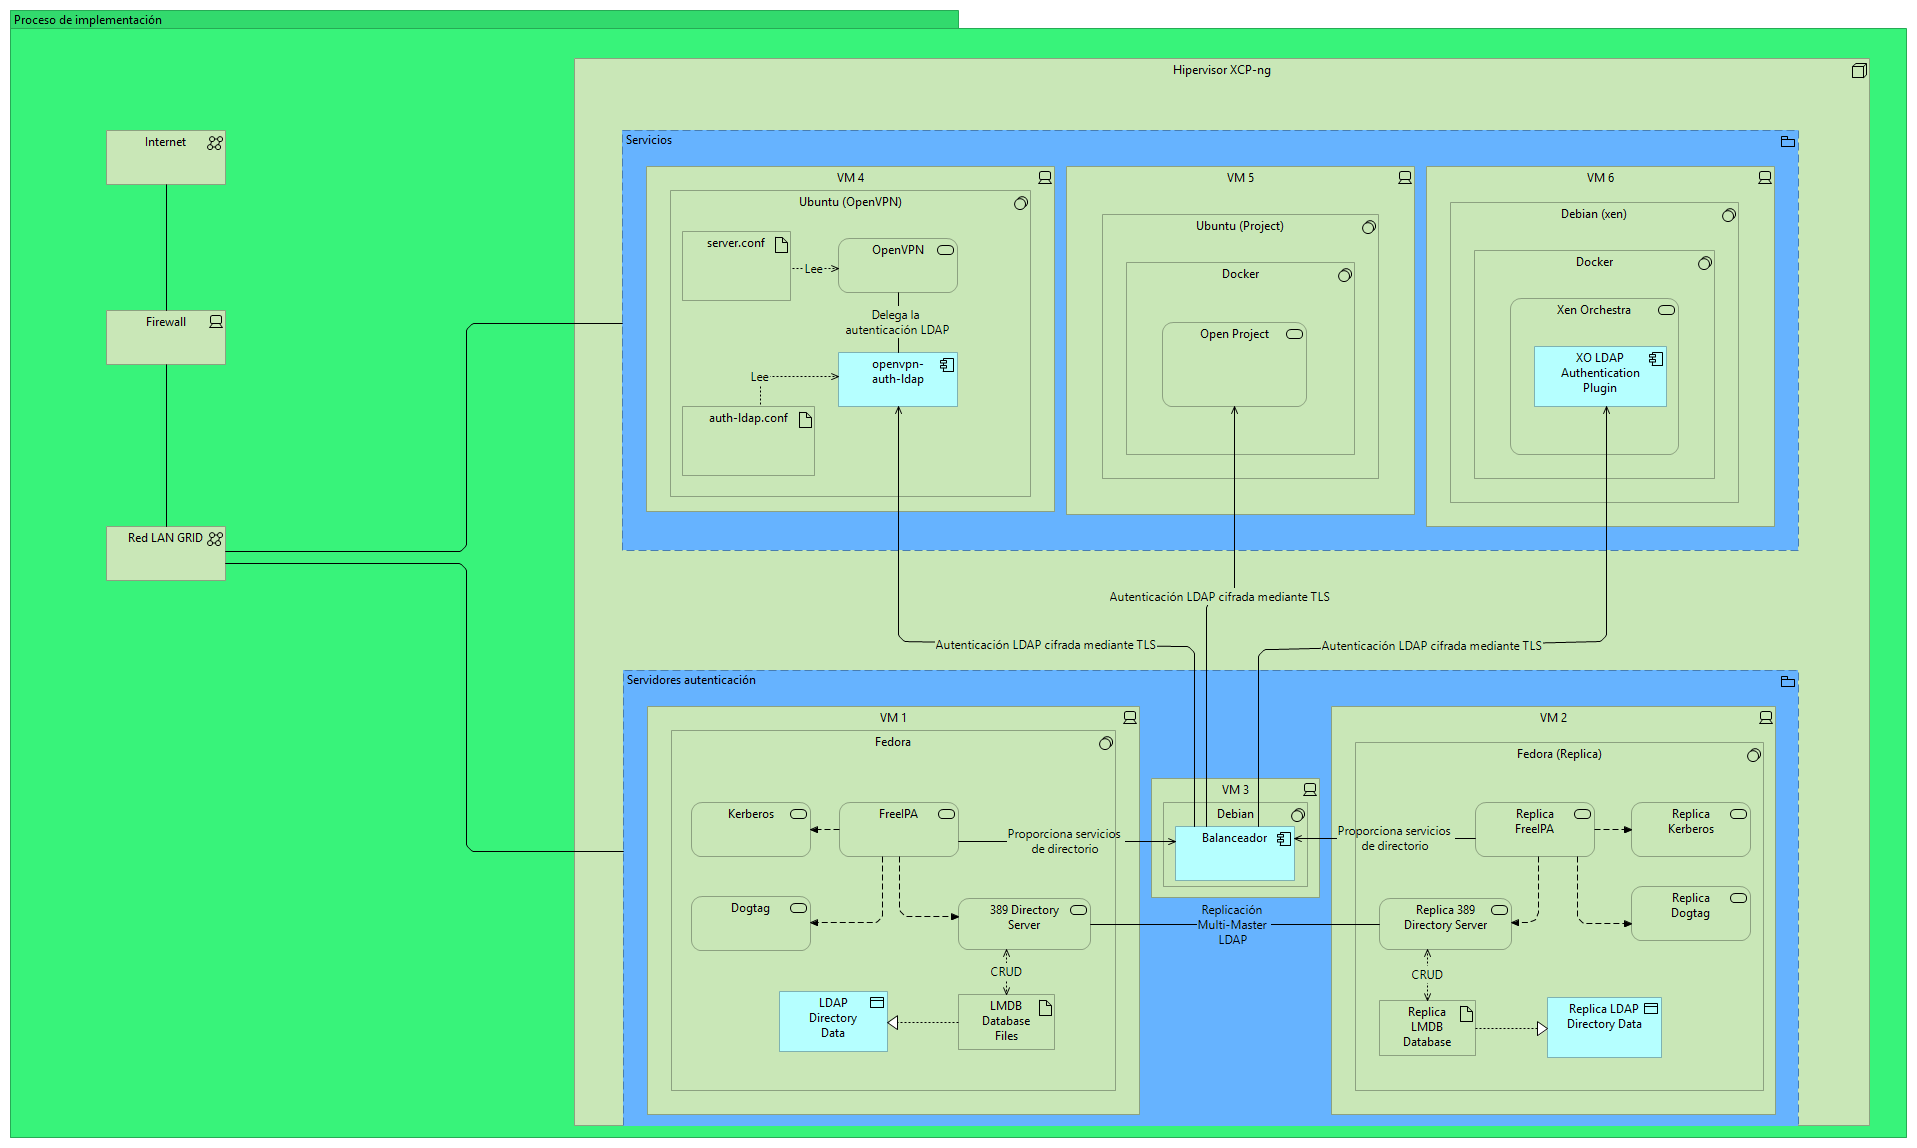
\includegraphics[width=0.9\textwidth]{imagenes/figuras/II-desarrollo-metodologico/disenio/implementation.png}
	\caption{vista de implementación}
	\label{fig:implementation}
\end{figure}

\subsection{Capa de infraestructura}

La \autoref{fig:infraestructure} presenta la infraestructura física y de red sobre la cual se despliega la solución propuesta. En ella se observa la conectividad desde Internet hacia la red institucional de la Universidad del Quindío mediante un acceso seguro, así como la integración con la infraestructura del \ac{GRID}. El entorno de ejecución está soportado por un servidor físico que actúa como hipervisor, sobre el cual se alojan las máquinas virtuales que conforman la solución. Esta arquitectura proporciona una plataforma centralizada para el despliegue y administración de los servicios, garantizando la comunicación entre los diferentes componentes y ofreciendo una base escalable para futuras ampliaciones de la infraestructura.

\begin{figure}[H]
	\centering
	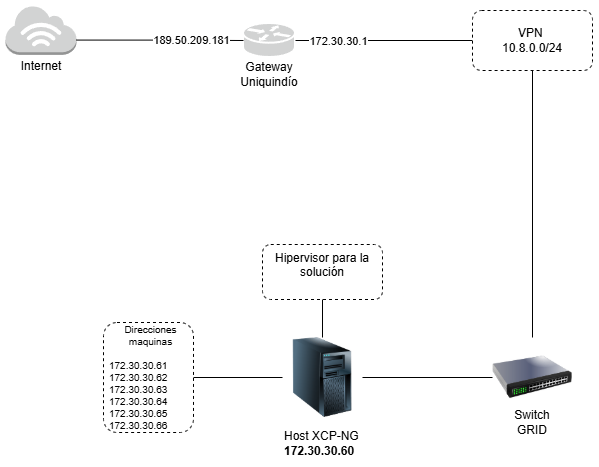
\includegraphics[width=0.9\textwidth]{imagenes/figuras/II-desarrollo-metodologico/disenio/infraestructure.png}
	\caption{vista de infraestructura}
	\label{fig:infraestructure}
\end{figure}

\subsection{Capa de virtualización}

La \autoref{fig:virtualization} presenta la vista de virtualización, cuyo propósito es representar la distribución de las máquinas virtuales que conforman la solución dentro de la plataforma de virtualización utilizada. Esta vista permite identificar la organización de los recursos virtualizados, los sistemas operativos implementados y la ubicación lógica de cada uno de los servicios que integran la arquitectura.

La solución se encuentra desplegada sobre un hipervisor de tipo 1 XCP-ng, instalado directamente sobre el servidor físico, lo que proporciona un entorno de virtualización con acceso directo a los recursos de hardware, mejorando el rendimiento, la disponibilidad y el aislamiento entre las diferentes cargas de trabajo. Sobre esta plataforma se ejecutan seis máquinas virtuales, cada una destinada a un propósito específico dentro de la infraestructura.

Las dos primeras máquinas virtuales corresponden al servicio de directorio y están conformadas por un servidor principal FreeIPA y un servidor réplica FreeIPA, ambos implementados sobre el sistema operativo Fedora. Esta configuración permite disponer de redundancia en el servicio FreeIPA mediante la replicación y sincronización de la información del directorio entre ambos servidores, favoreciendo la continuidad del servicio de autenticación ante la indisponibilidad de uno de ellos. La sexta máquina virtual corresponde al balanceador de carga, cuya función es distribuir las solicitudes entre los servicios que requieren un único punto de acceso y que no cuentan con mecanismos propios de failover mediante servidores alternativos.

\begin{figure}[H]
	\centering
	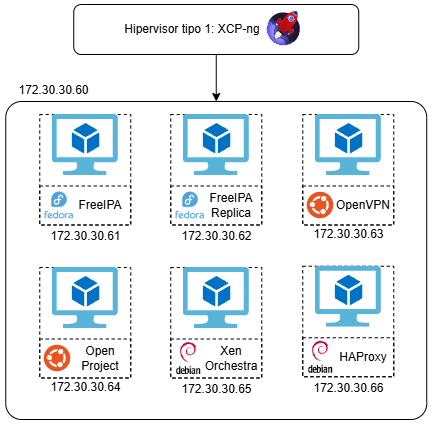
\includegraphics[width=0.9\textwidth]{imagenes/figuras/II-desarrollo-metodologico/disenio/virtualization.png}
	\caption{vista de virtualización}
	\label{fig:virtualization}
\end{figure}

\subsection{Vista por capas}

La \autoref{fig:layers} presenta la vista por capas de la arquitectura, cuyo propósito es proporcionar una visión integral de la solución propuesta, mostrando la relación existente entre las capas de negocio, aplicación e infraestructura. Esta vista permite comprender cómo los requerimientos funcionales de la organización son soportados por los componentes de software y cómo estos, a su vez, son desplegados sobre la infraestructura tecnológica.

En la capa de negocio se representan los actores involucrados en la administración y consumo del servicio de directorio, distinguiendo al Administrador de \ac{TI}, responsable de la gestión de identidades, y a los usuarios finales, representados por estudiantes y docentes, quienes consumen el servicio de autenticación centralizada. Asimismo, se identifican los servicios de negocio encargados de la administración de políticas, usuarios y grupos, además del servicio de autenticación y autorización que soporta el acceso a los recursos institucionales.

La capa de aplicación muestra la estructura lógica de FreeIPA y los componentes que cooperan para ofrecer los servicios de identidad. El 389 Directory Server actúa como repositorio central de usuarios, grupos y políticas; Kerberos proporciona los mecanismos de autenticación; Dogtag administra los certificados digitales; Policy Engine evalúa las reglas de autorización; y Web \acs{UI} + \ac{API} ofrece la interfaz para la administración del directorio. La interacción entre estos componentes permite implementar una plataforma unificada para la gestión de identidades y el control de acceso.

Finalmente, la capa de infraestructura representa el entorno sobre el cual se despliega la solución. En esta se observa un servidor físico que ejecuta un hipervisor encargado de alojar dos máquinas virtuales: una correspondiente al servidor principal de FreeIPA y otra destinada a la réplica del servicio. Ambas mantienen un mecanismo de replicación que garantiza la sincronización de la información del directorio y mejora la disponibilidad del servicio frente a posibles fallos.

Las relaciones entre las diferentes capas evidencian la trazabilidad de la arquitectura. Los servicios de negocio delegan la gestión de identidades y la autenticación en los componentes de FreeIPA, mientras que estos son soportados por la infraestructura de virtualización donde se encuentran desplegados el servidor principal y el servidor réplica. De esta manera, la vista demuestra cómo la arquitectura propuesta integra los objetivos del negocio con la implementación tecnológica, asegurando una solución centralizada, segura y con capacidad de alta disponibilidad para la administración de identidades del Grupo de Investigación \ac{GRID}.

\begin{figure}[H]
	\centering
	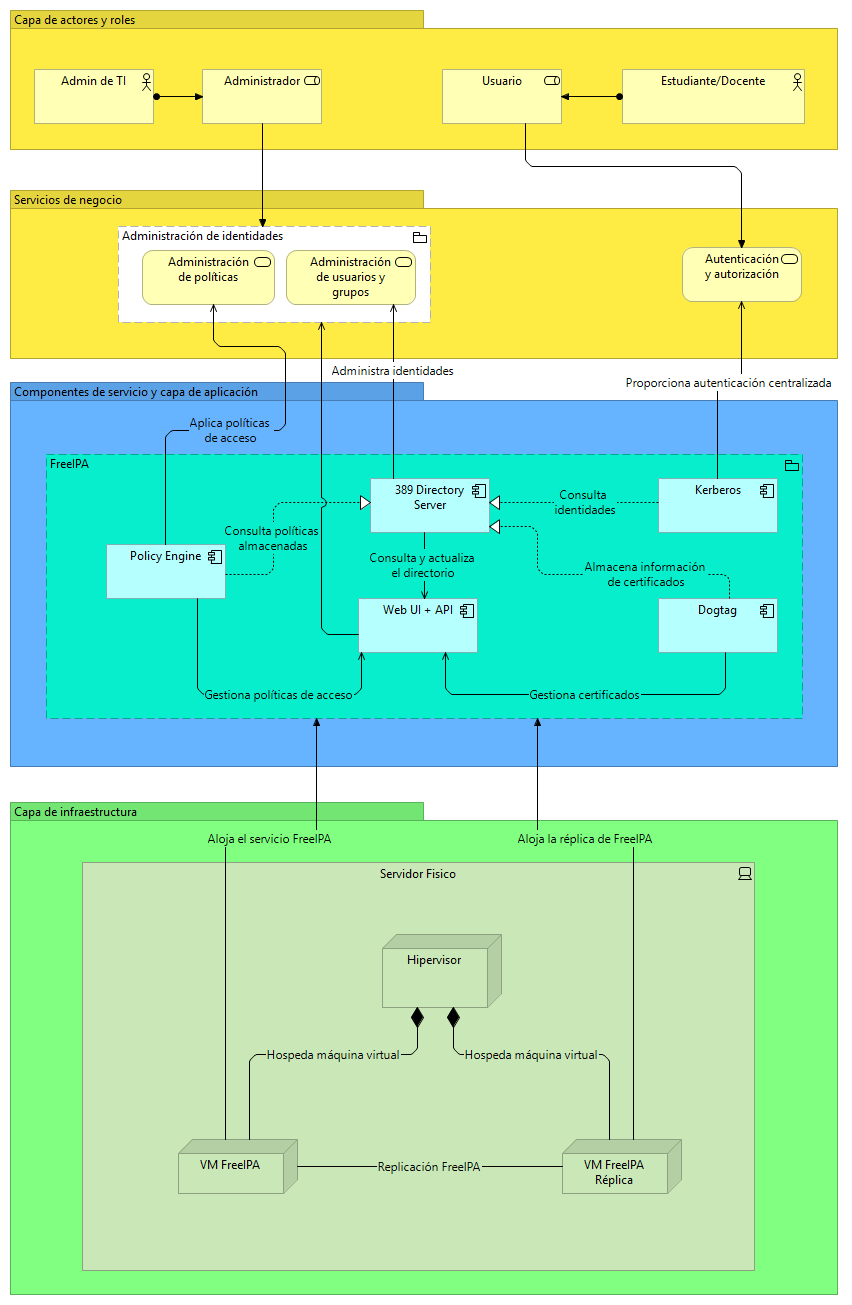
\includegraphics[width=0.9\textwidth]{imagenes/figuras/II-desarrollo-metodologico/disenio/layers.png}
	\caption{vista por capas}
	\label{fig:layers}
\end{figure}

\section{Diseño de configuraciones}\label{sec:diseno-configuraciones}

\subsection{Política de contraseñas}

Como parte del diseño del servicio de directorio se definió una política de contraseñas centralizada que será aplicada por FreeIPA sobre todas las identidades administradas por la plataforma. El propósito de esta política es establecer requisitos mínimos para la creación, utilización y administración de credenciales, garantizando un nivel homogéneo de seguridad para los servicios OpenVPN, Xen Orchestra y OpenProject integrados en la infraestructura del grupo de investigación \ac{GRID}.

La definición de la política se fundamenta en los controles establecidos por la norma ISO/IEC 27002:2022, particularmente en los controles 5.17 Información de autenticación (Authentication Information) y 8.5 Autenticación segura (Secure Authentication), los cuales establecen que las organizaciones deben implementar mecanismos para proteger las credenciales de autenticación mediante reglas de creación, distribución, almacenamiento, renovación y protección frente a intentos de acceso no autorizados.

Considerando las necesidades identificadas durante la fase de análisis, donde se evidenció la ausencia de un estándar institucional para la gestión de contraseñas y la necesidad de adoptar políticas alineadas con estándares internacionales, se definieron los parámetros presentados en la \autoref{tab:password-params}.

\begingroup
\fontsize{8.5pt}{9.5pt}\selectfont
\renewcommand{\arraystretch}{1.3}
\setlength{\tabcolsep}{4pt}

\begin{longtable}{|
>{\raggedright\arraybackslash}p{2.8cm}|
>{\raggedright\arraybackslash}p{3.5cm}|
>{\raggedright\arraybackslash}p{7.2cm}|}

\caption{Especificación de parámetros}
\label{tab:password-params}
\\
\hline
\textbf{Parámetro}                  &
\textbf{Valor definido}             &
\textbf{Justificación}
\\
\hline
\endfirsthead

\hline
\textbf{Parámetro}                  &
\textbf{Valor definido}             &
\textbf{Justificación}
\\
\hline
\endhead

Longitud mínima                     &
12 caracteres                       &
Incrementa la entropía de las credenciales y dificulta ataques por fuerza bruta.
\\
\hline

Complejidad                         &
Al menos una letra mayúscula, una letra minúscula, un número y un carácter especial &
Reduce la probabilidad de contraseñas predecibles y mejora su resistencia frente a ataques de diccionario.
\\
\hline

Historial de contraseñas            &
5 contraseñas                       &
Evita la reutilización inmediata de credenciales previamente utilizadas.
\\
\hline

Antigüedad mínima                   &
1 día                               &
Impide el cambio reiterado de contraseñas con el propósito de eludir el historial configurado.
\\
\hline

Vigencia máxima                     &
180 días                            &
Favorece la renovación periódica de credenciales sin generar una carga excesiva para los usuarios.
\\
\hline

Intentos fallidos                   &
5                                   &
Reduce el riesgo de ataques automatizados por fuerza bruta.
\\
\hline

Bloqueo de cuenta                   &
5 minutos                           &
Mitiga intentos reiterados de autenticación sin afectar significativamente la disponibilidad del servicio.
\\
\hline

Contraseña temporal                 &
Cambio obligatorio en el primer inicio de sesión &
Garantiza que únicamente el usuario conozca su contraseña definitiva.
\\
\hline

Auditoría                           &
Registro de autenticaciones, cambios de contraseña, bloqueos y restablecimientos &
Permite la trazabilidad de eventos y facilita los procesos de auditoría y respuesta ante incidentes.
\\
\hline
\endlongtable
\endgroup
\normalsize % Restablece explícitamente el tamaño de letra para el texto posterior

Los valores definidos no corresponden a requisitos explícitos establecidos por la norma ISO/IEC 27002:2022, ya que esta específica controles y buenas prácticas, pero no prescribe parámetros concretos como la longitud mínima de las contraseñas o el número máximo de intentos fallidos. En consecuencia, dichos valores fueron determinados como decisiones de diseño considerando las capacidades de configuración ofrecidas por FreeIPA, las recomendaciones internacionales para sistemas de gestión de identidades y el nivel de riesgo identificado para la infraestructura del grupo de investigación \ac{GRID}.

La implementación de esta política permitirá que todos los servicios integrados al directorio compartan un mismo conjunto de reglas de autenticación, eliminando las diferencias existentes entre plataformas y fortaleciendo la gestión centralizada de identidades, la protección de las credenciales y la trazabilidad de los accesos.

\subsection{Diseño del modelo de identidades}

Como parte del diseño del servicio de directorio, es necesario definir la estructura lógica de las identidades que serán administradas por FreeIPA. Esta estructura establece la organización de los usuarios, grupos y cuentas de servicio que posteriormente serán utilizados por las aplicaciones integradas para llevar a cabo los procesos de autenticación y autorización. De esta manera, se garantiza que la administración de identidades permanezca centralizada y que los diferentes servicios consuman una fuente única de información.

\subsubsection{Definición del nombre de dominio y del \texorpdfstring{\acs{FQDN}}{FQDN}}

Aunque FreeIPA puede integrar un servicio \ac{DNS}, en la presente implementación dicho componente no será utilizado. No obstante, FreeIPA requiere la definición de un nombre de dominio y de un Nombre de Dominio Completamente Calificado (Fully Qualified Domain Name, \ac{FQDN}) para el servidor principal, ya que estos identificadores son utilizados por \ac{LDAP}, Kerberos y la infraestructura de certificados digitales para identificar de forma única al servidor y emitir los principales de servicio correspondientes.

Para la infraestructura del grupo \ac{GRID} se definieron los parámetros presentados en la \autoref{tab:parametros-implementacion}.

\begingroup
\fontsize{8.5pt}{9.5pt}\selectfont
\renewcommand{\arraystretch}{1.3}
\setlength{\tabcolsep}{4pt}

\begin{longtable}{|
>{\raggedright\arraybackslash}p{2.8cm}|
>{\raggedright\arraybackslash}p{3.8cm}|
>{\raggedright\arraybackslash}p{6.9cm}|}

\caption{Parámetros para la implementación.}
\label{tab:parametros-implementacion}
\\
\hline
\textbf{Parámetro}                  &
\textbf{Valor definido}             &
\textbf{Justificación}
\\
\hline
\endfirsthead

\hline
\textbf{Parámetro}                  &
\textbf{Valor definido}             &
\textbf{Justificación}
\\
\hline
\endhead

Dominio \acs{DNS}                         &
grid.\allowbreak uniquindio.\allowbreak edu.\allowbreak co &
Corresponde al dominio institucional existente de la infraestructura \ac{GRID}. Este dominio ya es administrado por el servicio \ac{DNS} institucional y únicamente es referenciado por FreeIPA para la construcción de las identidades y de la estructura del directorio.
\\
\hline

Dominio \acs{LDAP} (Base \acs{DN})              &
dc=grid,\allowbreak dc=uniquindio,\allowbreak dc=edu,\allowbreak dc=co &
Se deriva directamente del dominio \ac{DNS}, donde cada componente del nombre de dominio se representa mediante un componente de dominio (Domain Component, dc), conforme al modelo de organización jerárquica utilizado por \ac{LDAP}.
\\
\hline

\acs{FQDN} del servidor                   &
ipa1.\allowbreak grid.\allowbreak uniquindio.\allowbreak edu.\allowbreak co &
Identifica de manera única al servidor FreeIPA dentro de la infraestructura. Este nombre es utilizado por Kerberos para generar los principales de servicio, por la autoridad certificadora para emitir los certificados digitales y por los clientes para establecer conexiones seguras con los servicios proporcionados por FreeIPA.
\\
\hline
\endlongtable
\endgroup
\normalsize % Restablece explícitamente el tamaño de letra para el texto posterior

La selección de estos valores garantiza la coherencia entre los servicios que conforman FreeIPA y evita inconsistencias durante los procesos de autenticación, emisión de certificados y establecimiento de conexiones seguras entre clientes y servidores.

\subsubsection{Definición de la estructura del directorio \texorpdfstring{\acs{LDAP}}{LDAP}}

Una vez definido el dominio de la infraestructura, es necesario establecer la organización lógica de los objetos que serán administrados por FreeIPA. Esta organización corresponde al Árbol de Información del Directorio (Directory Information Tree, \ac{DIT}), el cual define la disposición jerárquica de usuarios, grupos y demás objetos almacenados dentro del servicio \ac{LDAP}.

En la solución propuesta se adopta la estructura predeterminada de FreeIPA, la cual organiza los objetos administrativos bajo el contenedor cn=accounts. Esta organización facilita la administración de identidades y proporciona una estructura consistente para las consultas realizadas por las aplicaciones integradas.

\autoref{fig:directory-tree} presenta la estructura lógica del directorio utilizada en la solución.

\begin{figure}[H]
	\centering
	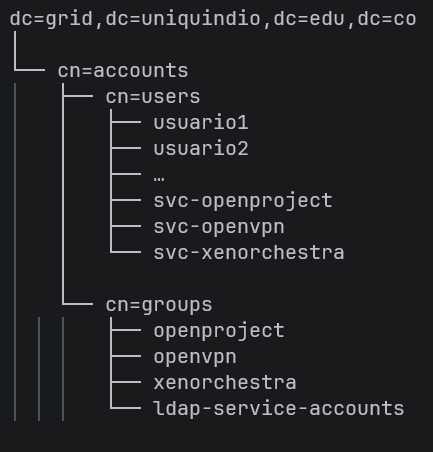
\includegraphics[width=0.9\textwidth]{imagenes/figuras/II-desarrollo-metodologico/disenio/directory-tree.png}
	\caption{árbol del directorio}
	\label{fig:directory-tree}
\end{figure}

La raíz del árbol corresponde al dominio \ac{LDAP} dc=grid,dc=uniquindio,dc=edu,dc=co, obtenido a partir del dominio institucional. Bajo esta raíz, FreeIPA agrupa los objetos relacionados con la administración de identidades dentro del contenedor cn=accounts.

El contenedor cn=users almacena tanto las cuentas de los usuarios finales como las cuentas de servicio utilizadas por las aplicaciones para realizar consultas \ac{LDAP}. Por su parte, el contenedor cn=groups reúne los grupos empleados para implementar los mecanismos de autorización de los servicios y para administrar las políticas aplicadas a las cuentas de servicio.

Esta organización constituye la base sobre la cual las aplicaciones realizan las búsquedas \ac{LDAP}. Por ejemplo, los servicios integrados utilizan el contenedor cn=users como punto de partida para localizar usuarios, mientras que la pertenencia a los grupos definidos en cn=groups permite determinar los permisos de acceso correspondientes a cada aplicación.

\subsubsection{Definición de grupos de autorización}

Con el propósito de centralizar la administración del acceso a las aplicaciones integradas, se definieron grupos específicos dentro del directorio para cada uno de los servicios que consumen información desde FreeIPA. En lugar de asignar permisos individualmente a cada usuario, el acceso a las aplicaciones se determina mediante la pertenencia a dichos grupos.

\autoref{tab:grupos-autorizacion} presenta los grupos definidos para la solución

\begingroup
\fontsize{8.5pt}{9.5pt}\selectfont
\renewcommand{\arraystretch}{1.3}
\setlength{\tabcolsep}{4pt}

\begin{longtable}{|
>{\raggedright\arraybackslash}p{2.8cm}|
>{\raggedright\arraybackslash}p{3.5cm}|
>{\raggedright\arraybackslash}p{7.2cm}|}

\caption{Grupos de autorización.}
\label{tab:grupos-autorizacion}
\\
\hline
\rowcolor[gray]{0.85}
\textbf{Grupo}                  &
\textbf{Servicio asociado}     &
\textbf{Propósito}
\\
\hline
\endfirsthead

\hline
\rowcolor[gray]{0.85}
\textbf{Grupo}                  &
\textbf{Servicio asociado}     &
\textbf{Propósito}
\\
\hline
\endhead

openproject                         &
OpenProject                         &
Autoriza el acceso a la plataforma de gestión de proyectos mediante autenticación \ac{LDAP}.
\\
\hline

openvpn                             &
OpenVPN                             &
Autoriza a los usuarios que pueden establecer conexiones \ac{VPN} con la infraestructura.
\\
\hline

xenorchestra                        &
Xen Orchestra                       &
Autoriza el acceso a la plataforma de administración de virtualización.
\\
\hline
\endlongtable
\endgroup
\normalsize

Cada servicio realiza consultas \ac{LDAP} filtrando los usuarios pertenecientes al grupo correspondiente, implementando un mecanismo de autorización basado en grupos. Esta estrategia simplifica la administración de permisos, ya que el alta o baja de un usuario únicamente requiere modificar su pertenencia al grupo respectivo sin necesidad de reconfigurar cada aplicación.

\subsubsection{Diseño de cuentas de servicio}

Las aplicaciones integradas requieren realizar consultas al directorio \ac{LDAP} para localizar la información del usuario y establecer el proceso de autenticación. Con este propósito se definieron cuentas de servicio, las cuales son utilizadas exclusivamente por las aplicaciones para establecer la conexión con el directorio y realizar operaciones de consulta. Estas cuentas poseen únicamente los privilegios necesarios para leer la información almacenada en el servicio de directorio, en concordancia con el principio de mínimo privilegio.

Con el fin de mejorar el aislamiento de credenciales y la trazabilidad de las operaciones realizadas sobre el directorio, se definió una cuenta de servicio independiente para cada una de las aplicaciones integradas. Esta estrategia permite administrar las credenciales de forma individual, de manera que un eventual compromiso o rotación de la contraseña de una cuenta no afecte el funcionamiento de los demás servicios.

\begingroup
\fontsize{8.5pt}{9.5pt}\selectfont
\renewcommand{\arraystretch}{1.3}
\setlength{\tabcolsep}{4pt}

\begin{longtable}{|
>{\raggedright\arraybackslash}p{6.0cm}|
>{\raggedright\arraybackslash}p{7.5cm}|}

\caption{Cuentas de servicio.}
\label{tab:cuentas-servicio}
\\
\hline
\rowcolor[gray]{0.85}
\textbf{Cuenta}                  &
\textbf{Servicio}
\\
\hline
\endfirsthead

\hline
\rowcolor[gray]{0.85}
\textbf{Cuenta}                  &
\textbf{Servicio}
\\
\hline
\endhead

svc-openproject                     &
OpenProject                         \\
\hline

svc-openvpn                         &
OpenVPN                             \\
\hline

svc-xenorchestra                    &
Xen Orchestra                       \\
\hline
\endlongtable
\endgroup
\normalsize

Con el propósito de simplificar la administración de las cuentas de servicio, todas ellas se agrupan en el grupo ldap-service-accounts. Sobre este grupo se aplica una política de contraseñas específica para cuentas de servicio, de modo que toda cuenta incorporada al grupo queda sujeta automáticamente a dicha política, sin necesidad de configurarla de forma individual.

Con el fin de garantizar que esta política prevalezca sobre la política global del dominio, se le asigna una prioridad numérica superior. De esta manera, cuando una cuenta pertenece al grupo ldap-service-accounts, FreeIPA aplica la política específica para cuentas de servicio en lugar de la política general utilizada para los usuarios finales.

La política de contraseñas definida para el grupo ldap-service-accounts se resume en la \autoref{tab:politica-service-accounts}


\begingroup
\fontsize{8.5pt}{9.5pt}\selectfont
\renewcommand{\arraystretch}{1.3}
\setlength{\tabcolsep}{4pt}

\begin{longtable}{|
>{\raggedright\arraybackslash}p{3.5cm}|
>{\raggedright\arraybackslash}p{10.0cm}|}

\caption{Política de contraseñas para el grupo ldap-service-accounts.}
\label{tab:politica-service-accounts}
\\
\hline
\rowcolor[gray]{0.85}
\textbf{Elemento}               &
\textbf{Descripción}
\\
\hline
\endfirsthead

\hline
\rowcolor[gray]{0.85}
\textbf{Elemento}               &
\textbf{Descripción}
\\
\hline
\endhead

Grupo                           &
ldap-service-accounts           \\
\hline

Propósito                       &
Agrupar las cuentas de servicio utilizadas por las aplicaciones integradas. \\
\hline

Miembros                        &
svc-openproject, svc-openvpn y svc-xenorchestra. \\
\hline

Política asociada              &
Política de contraseña para cuentas de servicio. \\
\hline

Prioridad                       &
10                              \\
\hline

Configuración principal        &
Contraseña sin expiración.      \\
\hline

Justificación                   &
Garantizar la disponibilidad continua de las integraciones sin afectar las políticas aplicadas a los usuarios finales. \\
\hline
\endlongtable
\endgroup
\normalsize

La utilización de un grupo dedicado para las cuentas de servicio permite centralizar la administración de las políticas de seguridad y facilita la incorporación de nuevas aplicaciones al servicio de directorio, ya que únicamente es necesario crear la cuenta correspondiente y asociarla al grupo definido.

En conjunto, la estructura del directorio, los grupos de autorización y las cuentas de servicio definen el modelo de gestión de identidades de la solución propuesta. Esta organización centraliza la administración de usuarios y credenciales, facilita la incorporación de nuevos servicios al directorio y establece la base sobre la cual se implementarán las integraciones \ac{LDAP} descritas en el capítulo de implementación.

\subsection{Definición de máquinas virtuales}

Con el fin de garantizar la disponibilidad y continuidad del servicio de directorio, la arquitectura propuesta contempla el despliegue de dos servidores FreeIPA: un servidor principal y un servidor réplica. Esta configuración permite mantener una copia sincronizada de la información de identidades, políticas y servicios de autenticación, proporcionando tolerancia a fallos y continuidad operativa en caso de indisponibilidad de uno de los servidores.

Ambas máquinas virtuales fueron diseñadas con características de hardware homogéneas para asegurar un comportamiento consistente durante los procesos de replicación y administración del servicio. Asimismo, los dos servidores ejecutan la misma distribución del sistema operativo y la misma versión de FreeIPA, reduciendo posibles problemas de compatibilidad durante la sincronización de datos. Las especificaciones técnicas de cada servidor FreeIPA se presentan en la \autoref{tab:ficha-servidor-principal} y la \autoref{tab:ficha-servidor-replica}.

\begingroup
\fontsize{8.5pt}{9.5pt}\selectfont
\renewcommand{\arraystretch}{1.3}
\setlength{\tabcolsep}{4pt}

\begin{longtable}{|
	>{\raggedright\arraybackslash}p{4.0cm}|
	>{\raggedright\arraybackslash}p{9.5cm}|}

	\caption{Ficha técnica del servidor principal FreeIPA}
	\label{tab:ficha-servidor-principal}
	\\
	\hline
	\rowcolor[gray]{0.85}
	\textbf{Característica}      &
	\textbf{Especificación}
	\\
	\hline
	\endfirsthead

	\hline
	\rowcolor[gray]{0.85}
	\textbf{Característica}      &
	\textbf{Especificación}
	\\
	\hline
	\endhead

	Nombre de la máquina         & ipa1                                                                        \\ \hline
	Función                      & Servidor principal FreeIPA                                                  \\ \hline
	Sistema operativo            & Fedora Server 44                                                            \\ \hline
	Plataforma de virtualización & XCP-ng                                                                      \\ \hline
	vCPU                         & 2                                                                           \\ \hline
	Memoria \acs{RAM}                  & 4 \acs{GB}                                                                        \\ \hline
	Almacenamiento               & 50 \acs{GB}                                                                       \\ \hline
	Dirección \acs{IP}                 & 172.30.30.61                                                                \\ \hline
	Nombre virtual               & ipa.\allowbreak grid.\allowbreak uniquindio.\allowbreak edu.\allowbreak co  \\ \hline
	Nombre de dominio (\acs{FQDN})     & ipa1.\allowbreak grid.\allowbreak uniquindio.\allowbreak edu.\allowbreak co \\ \hline
	Dominio IPA                  & grid.\allowbreak uniquindio.\allowbreak edu.\allowbreak co                  \\ \hline
	Reino Kerberos               & \acs{GRID}.\allowbreak UNIQUINDIO.\allowbreak EDU.\allowbreak CO                  \\ \hline
\end{longtable}
\endgroup
\normalsize

\begingroup
\fontsize{8.5pt}{9.5pt}\selectfont
\renewcommand{\arraystretch}{1.3}
\setlength{\tabcolsep}{4pt}

\begin{longtable}{|
	>{\raggedright\arraybackslash}p{4.0cm}|
	>{\raggedright\arraybackslash}p{9.5cm}|}

	\caption{Ficha técnica del servidor réplica FreeIPA}
	\label{tab:ficha-servidor-replica}
	\\
	\hline
	\rowcolor[gray]{0.85}
	\textbf{Característica}      &
	\textbf{Especificación}
	\\
	\hline
	\endfirsthead

	\hline
	\rowcolor[gray]{0.85}
	\textbf{Característica}      &
	\textbf{Especificación}
	\\
	\hline
	\endhead

	Nombre de la máquina         & ipa2                                                                        \\ \hline
	Función                      & Servidor réplica FreeIPA                                                    \\ \hline
	Sistema operativo            & Fedora Server 44                                                            \\ \hline
	Plataforma de virtualización & XCP-ng                                                                      \\ \hline
	vCPU                         & 2                                                                           \\ \hline
	Memoria \acs{RAM}                  & 4 \acs{GB}                                                                        \\ \hline
	Almacenamiento               & 50 \acs{GB}                                                                       \\ \hline
	Dirección \acs{IP}                 & 172.30.30.62                                                                \\ \hline
	Nombre virtual               & ipa.\allowbreak grid.\allowbreak uniquindio.\allowbreak edu.\allowbreak co  \\ \hline
	Nombre de dominio (\acs{FQDN})     & ipa2.\allowbreak grid.\allowbreak uniquindio.\allowbreak edu.\allowbreak co \\ \hline
	Dominio IPA                  & grid.\allowbreak uniquindio.\allowbreak edu.\allowbreak co                  \\ \hline
	Reino Kerberos               & \acs{GRID}.\allowbreak UNIQUINDIO.\allowbreak EDU.\allowbreak CO                  \\ \hline
\end{longtable}
\endgroup
\normalsize

Las características de hardware de los servidores FreeIPA fueron seleccionadas considerando los requerimientos operacionales del grupo de investigación \ac{GRID}, el número esperado de usuarios y servicios integrados, así como las recomendaciones generales para despliegues de FreeIPA en entornos de pequeña y mediana escala. La utilización de una réplica proporciona redundancia del servicio de directorio, replicación automática de la información de identidades y una mayor disponibilidad de los mecanismos de autenticación centralizada, contribuyendo a mejorar la resiliencia de la infraestructura propuesta.

Adicionalmente, durante la implementación fue necesario incorporar una tercera máquina virtual destinada a ejecutar HAProxy. Esta máquina no forma parte del servicio de directorio ni participa en el proceso de replicación de FreeIPA; su función consiste en proporcionar un punto de acceso unificado hacia los servidores del directorio. De esta manera, los servicios integrados pueden utilizar un único punto de conexión en lugar de depender directamente de la dirección de uno de los servidores FreeIPA.

La incorporación de HAProxy permite centralizar el acceso a los servidores de directorio y facilita la distribución de las conexiones entre el servidor principal y la réplica. Asimismo, esta configuración permite mantener un único dominio de acceso para los servicios que requieren autenticación mediante \ac{LDAP}, evitando que cada servicio deba conocer individualmente la dirección de los servidores que conforman la infraestructura de FreeIPA.

Las especificaciones técnicas de la máquina virtual destinada a HAProxy se presentan en la \autoref{tab:ficha-servidor-haproxy}.
\begingroup
\fontsize{8.5pt}{9.5pt}\selectfont
\renewcommand{\arraystretch}{1.3}
\setlength{\tabcolsep}{4pt}

\begin{longtable}{|
	>{\raggedright\arraybackslash}p{4.0cm}|
	>{\raggedright\arraybackslash}p{9.5cm}|}

	\caption{Ficha técnica del servidor HAProxy}
	\label{tab:ficha-servidor-haproxy}
	\\
	\hline
	\rowcolor[gray]{0.85}
	\textbf{Característica}      &
	\textbf{Especificación}
	\\
	\hline
	\endfirsthead

	\hline
	\rowcolor[gray]{0.85}
	\textbf{Característica}      &
	\textbf{Especificación}
	\\
	\hline
	\endhead

	Nombre de la máquina         & haproxy                                                               \\ \hline
	Función                      & Proxy inverso y punto de acceso unificado para los servidores FreeIPA \\ \hline
	Sistema operativo            & Debian 12                                                             \\ \hline
	Plataforma de virtualización & XCP-ng                                                                \\ \hline
	vCPU                         & 2                                                                     \\ \hline
	Memoria \acs{RAM}                  & 2 \acs{GB}                                                                  \\ \hline
	Almacenamiento               & 20 \acs{GB}                                                                 \\ \hline
\end{longtable}
\endgroup
\normalsize
